\documentclass[en]{university}

\faculty{Department of Computer Engineering}
\course{Artificial Intelligence}
\subject{Mini Project 4 Theory Questions}
\professor{Dr. Rohban}
\student{Parsa Mohammadian}

\begin{document}

\setupdocument

\section{}

\subsection{}

\includepdfall{assets/1a.pdf}

\subsection{}

We can use introduced features as nodes of the decision tree, and values (black and white) as the edges of the decision tree. But 
this structure is extremely over fitted to the data. We can traverse resulting tree to classify the input image $X$ but it is not 
accurate.

\section{}

First we should consider our training data can be separated by a hyperplane, then we prove perceptron algorithm convergence for this kind of data.

We define \textbf{maximum margin} $\delta$ as the distance between the best hyperplane and the nearest point of the training data.

$$
    \delta = \max_w min_{(x_i, y_i)} [y_i w^T x_i] \text{ such that, } ||w||_2 = 1
$$

Let $\hat{w}$ be the best separating hyperplane with margin $\delta$, $w^{(k)}$ be the weights of the $k^{th}$ iteration starting 
from the zero vector, and $\theta$ be the angle between these two vectors. 
We want $w^{(k)}$ get near to $\hat{w}$ in each iteration and finally converge to $\hat{w}$. We can show that 
by illustrating the convergence of $\cos(\theta)$ to one, or in other words, $\theta$ convergence to zero.

We also divide all the training data by $\max[||y_i x_i||]$ to normalize the data. Hence, we can say 
$\forall i : ||y_i x_i||_2^2 \leq 1$.

\begin{gather*}
    ||w^{(k)}||_2^2 = ||w^{(k-1)} + y_i x_i||_2^2 \\
    = ||w^{(k-1)}||_2^2 + ||y_i x_i||_2^2 + 2 y_i w^T x_i \\
    y_i w^(k-1)T x_i < 0 \text{ because update rule } \\
    \Rightarrow ||w^{(k)}||_2^2 \leq ||w^{(k-1)}||_2^2 + \underbrace{||y_i x_i||_2^2}_{\leq 1} \\
    \leq ||w^{(k-1)}||_2^2 + 1 \\
    \text{ By solving this recursive inequality, we can show that } ||w^{(k)}||_2^2 \leq k \\
    \Rightarrow ||w^{(k)}||_2 \leq \sqrt{k}
\end{gather*}

So we have found an upper bound for the norm of the weights in each iteration.

\begin{gather*}
    \hat{w} \cdot w^{(k)} = \hat{w}^T w^{(k)} \\
    = \hat{w}^T (w^{(k-1)} + y_i x_i) \\
    = \hat{w}^T w^{(k-1)} + \underbrace{\hat{w}^T y_i x_i}_{\geq \delta} \\
    \geq \hat{w}^T w^{(k-1)} + \delta \\
    \text{ By solving this recursive inequality, we can show that } \hat{w} \cdot w^{(k)} \geq k \delta 
\end{gather*}

Here is a lower bound for $\hat{w} \cdot w^{(k)}$.

\begin{gather*}
    \begin{cases}
        ||w^{(k)}||_2 \leq \sqrt{k} \\
        \hat{w} \cdot w^{(k)} \geq k \delta 
    \end{cases} \\
    \Rightarrow \underbrace{||w^{(k)}||_2}_{\leq \sqrt{k}} \underbrace{||\hat{w}||_2}_{1} \cos(\theta) \geq \sqrt{k} \delta \\
    \Rightarrow \cos(\theta) \geq \frac{k \delta}{\sqrt{k}} \\
    \Rightarrow \cos(\theta) \geq \sqrt{k} \delta \\
    \text{Suppose we choose } k = \frac{1}{\delta^2} \Rightarrow \cos(\theta) \geq 1 \\
    \text{ So } \cos(\theta) \text{ is convergent to } 1
\end{gather*}

So for $k = \lceil \frac{1}{\delta^2} \rceil$ iterations, the perceptron algorithm will converge to the best separating hyperplane.

\section{}

Since perceptron is a linear classifier, we can introduce an neural network consisting of multiple layer of perceptrons for the given shape. 
First we find the weights and biases of the first layer of perceptrons as shown in figure \ref{fig:w}. Each $w_i, b_i$ is weight and bias 
of the $P_i$ perceptron in the first layer. Since equation for separator line is given by $w_i^(2) y = -w_i^(1) x + b_i$, we can find the weights
and biases of the first layer as bellow.

\begin{gather*}
    y = \frac{1}{2} x + 2 \Rightarrow w_1 = \begin{bmatrix}-\frac{1}{2} \\ 1\end{bmatrix}, b_1 = 2 \\
    y = 3 x - 3 \Rightarrow w_2 = \begin{bmatrix}-3 \\ 1\end{bmatrix}, b_2 = -3 \\
    y = - 3 x + 3 \Rightarrow w_3 = \begin{bmatrix}3 \\ 1\end{bmatrix}, b_3 = 3 \\
    y = - \frac{1}{2} x - 2 \Rightarrow w_4 = \begin{bmatrix}\frac{1}{2} \\ 1\end{bmatrix}, b_4 = -2 \\
    y = \frac{1}{2} x - 2 \Rightarrow w_5 = \begin{bmatrix}-\frac{1}{2} \\ 1\end{bmatrix}, b_5 = -2 \\
    y = 3 x + 3 \Rightarrow w_6 = \begin{bmatrix}-3 \\ 1\end{bmatrix}, b_6 = 3 \\
    y = -3 x - 3 \Rightarrow w_7 = \begin{bmatrix}3 \\ 1\end{bmatrix}, b_7 = -3 \\
    y = - \frac{1}{2} x + 2 \Rightarrow w_8 = \begin{bmatrix}\frac{1}{2} \\ 1\end{bmatrix}, b_8 = 2
\end{gather*}

\begin{figure}[!htbp]
\centering
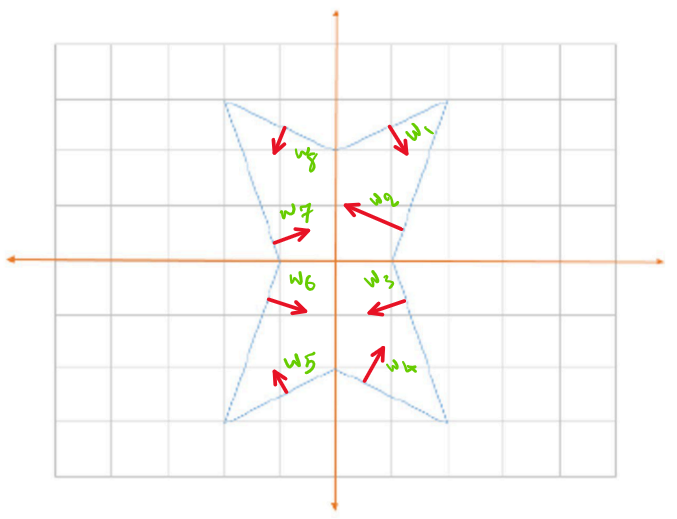
\includegraphics[width=1\textwidth]{assets/3w.png}
\caption{Weights and biases of the first layer of perceptrons}
\label{fig:w}
\end{figure}

We also use sign activation function after the first layer which graph is shown in figure \ref{fig:sign}.

\begin{figure}[!htbp]
    \centering
    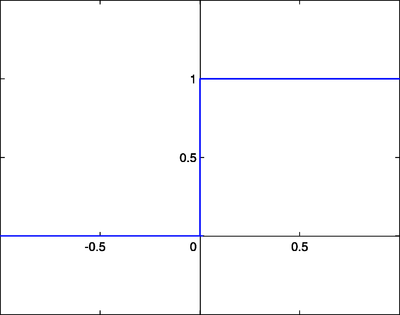
\includegraphics[width=1\textwidth]{assets/sign.png}    
    \caption{Sign activation function}
    \label{fig:sign}
\end{figure}

Given non-convex shape can be represented by 4 convex shape like the red one in figure \ref{fig:convex}. 
We can use these four convex shape in the second layer of perceptrons. Now we should find the weights and biases of the second layer of perceptrons. 
The intuition behind this is that we should get logical and of four lines which are the sides of each convex shape and ignore the other lines. 
We also use another sign activation function after the second layer.

\begin{gather*}
    c_1: w = \begin{bmatrix}
        1 \\
        1 \\
        0 \\
        0 \\
        1 \\
        0 \\
        1 \\
        0
    \end{bmatrix}, b = -3.5 --
    c_2: w = \begin{bmatrix}
        0 \\
        0 \\
        1 \\
        1 \\
        0 \\
        1 \\
        0 \\
        1
    \end{bmatrix}, b = -3.5 \\
    c_3: w = \begin{bmatrix}
        0 \\
        0 \\
        1 \\
        0 \\
        1 \\
        1 \\
        0 \\
        1
    \end{bmatrix}, b = 3.5 --
    c_4: w = \begin{bmatrix}
        0 \\
        1 \\
        0 \\
        0 \\
        1 \\
        0 \\
        1 \\
        1
    \end{bmatrix}, b = 3.5
\end{gather*}

\begin{figure}[!htbp]
\centering
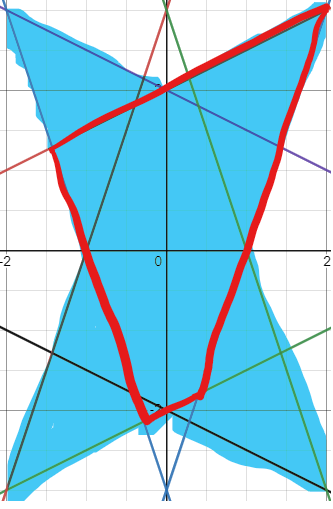
\includegraphics[width=1\textwidth]{assets/3convex.png}
\caption{Convex shapes of the second layer of perceptrons}
\label{fig:convex}
\end{figure}

At the last layer the intuition is that we should get logical or of four area, it means our point is in given shape if the point is at least in one 
of the four convex shapes. 

\begin{gather*}
    o: w = \begin{bmatrix}
        1 \\
        1 \\
        1 \\
        1 
    \end{bmatrix}, b = -0.5
\end{gather*}

Again we use sign activation function after the last layer. The whole neural network is shown in figure \ref{fig:n}.

\begin{figure}[!htbp]
\centering
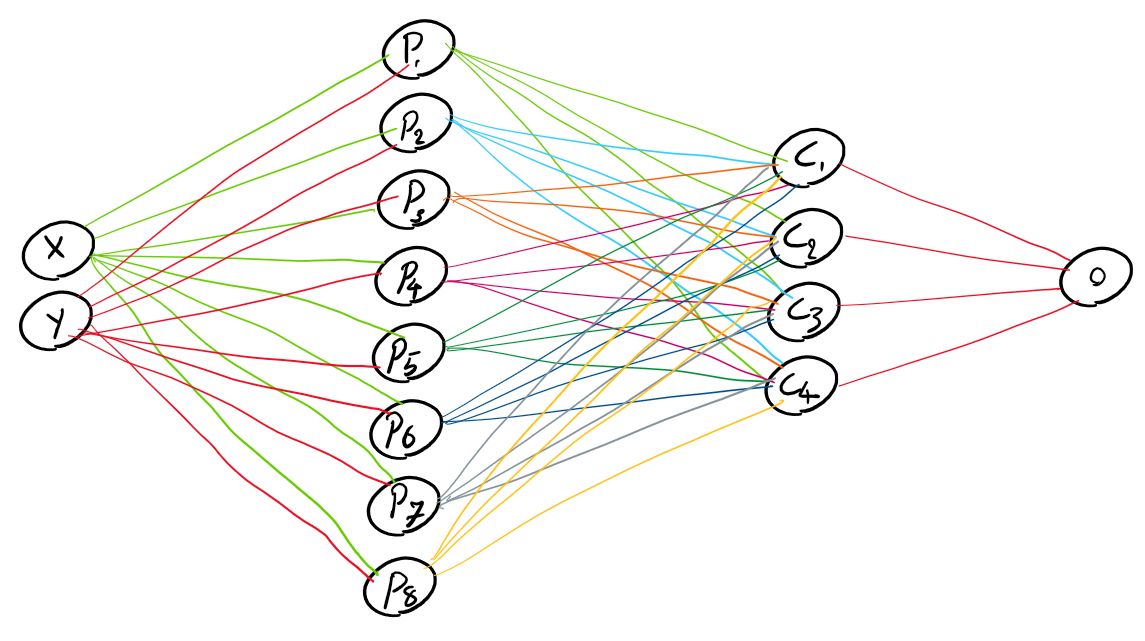
\includegraphics[width=1\textwidth]{assets/3n.png}
\caption{Neural network}
\label{fig:n}
\end{figure}

\end{document}